\chapter{Methodology - Preparation}
\label{sec:methodology_preparation}

As mentioned above the endeavor of this thesis was to put together a front to back landing procedure utilizing an existing vision based landing site detection pipeline and an autonomy framework. In order to do this, all individual software instances needed to be ready in order to combine them and achieve autonomous landing in unknown terrain.

\section{Stereo Camera Depth Perception} \label{sec:StereoDepth}

The autonomy framework\citep{Autonomy} allows us to fly independent missions at cruise altitude of 100m+. The structure from motion approach captures 3D information during traversal as its adaptive baseline allows it to perceive high quality depth information also at such high altitudes. This information can be used by LSD in order to detect landing sites during mission. 

At low altitudes SFM works as well but surrounded with obstacles, the need for lateral motion poses significant risk. This is because the drone does not retain any hazard information due to the limitations of computational complexity present for Mars flights. 

\subsection{Stereo Camera - SFM Comparison}

The specific advantage of a stereo camera implementation when compared to SFM can be summarized in the following points:

\begin{itemize}
    \item No necessity of lateral motion
    \item Hardware depth perception
    \item DEM converion
    \item Efficiency
\end{itemize}

\subsubsection{Lateral Motion}

As already mentioned above the need for lateral motion in itself is an undesirable necessity for a rotorcraft in unknown terrain. 

In this setup the structure from motion approach is based on a key frame buffer which needs to be filled with image-pose pairs at different horizontal positions in order to start acquiring depth information. The current setting in the implementation \citet{SFM} uses 6 key frames. Therefore, for a single point cloud it is necessary to move laterally 6 times in order to start perceiving depth. Following the depth error formula from a stereo disparity image (\ref{eq:SFM_depth_error}) and assuming an altitude of 2.5m above ground with a focal length of 256 pixels and a disparity error of 0.5 pixels, the necessary baseline in order to keep the depth error below a critical 5cm is:

\subsubsection{Software vs Hardware Depth Perception}

Structure from Motion, being a software node that relies on camera poses supplied by a state estimator, is by design subject to inaccuracies. A depth node based on a stereo camera on the other hand works with a fixed rigid baseline between the camera views. Thus, for low altitude flights that bear the danger of collision, a more robust hardware approach is preferred.

\subsubsection{DEM Conversion}

As described in \cref{subsubsec:setup:aggregation} the multi-resolution DEM used for depth aggregation in LSD is based on Optimal Mixture of Gaussian cells and thus converges over time. 

According to \cref{subsubsec:setup:haz_seg} the landing sites chosen are likely on terrain with low uncertainty. Because of this landing sites are more likely to be detected and have in general a better quality when the terrain perceived has been viewed.

When a landing site has been selected we need to make sure that the landing site is actually correctly detected and of good quality. For this we would like to (re-)detect landing sites on rather converged terrain. Structure from Motion needs constant lateral motion for this. A stereo camera depth node simply hovers in place for any given amount of time.

\subsubsection{Efficiency}

All in all the stereo camera setup allows us to perceive a landing site at course altitude and after having traversed horizontally to that location, we can simply descent to a stereo camera friendly altitude for the verification. Compared to repeated lateral coverage of the area in question this is a huge increase in efficiency.

\subsection{Theoretical Analysis}

When it comes to depth perception the obvious drawback of a stereo camera is its limited baseline. It only perceives depth accurately for objects within a certain proximity to the lense. 

Assuming a perfectly calibrated and rectified camera there is still always an inaccuracy in the depth estimation arising from the disparity error.

From a given disparity estimate the depth error is derived as follows:

\begin{equation}\label{eq:depth_from_disp}
    z = \frac{f \cdot b}{d}
\end{equation}

Where b is the z is the depth estimate, b is the baseline, f is the focal length and d is the disparity value.

Taking the derivative of z w.r.t. d we get

\begin{equation}
    \frac{\partial z}{\partial d} = - \frac{f  \cdot b}{z^2}
\end{equation}

And substituting (\cref{eq:depth_from_disp}) we get:

\begin{equation}
    {\partial z} = \frac{z^2}{f  \cdot b}\partial d
\end{equation}

Where the sign was left away as for our application there lies equal danger in a point being perceived too close and too far away.

For the maximum altitude given a maximum allowable depth error this yields:

\begin{equation}
    z_{\text{max}} = \sqrt{\frac{\Delta z_{\text{max}} \cdot b \cdot f}{\Delta d}}
\end{equation}

Where $\Delta z$ is the depth error and $\Delta d$ the disparity error.

The stereo camera mounted on the drone in JPL's aerial vehicle lab had a baseline of about 10cm and a focal length of 256.

With these properties and estimating a subpixel precision disparity error of 0.5 pixels the depth error at varying altitudes looks as follows:

\begin{figure}
    \centering
    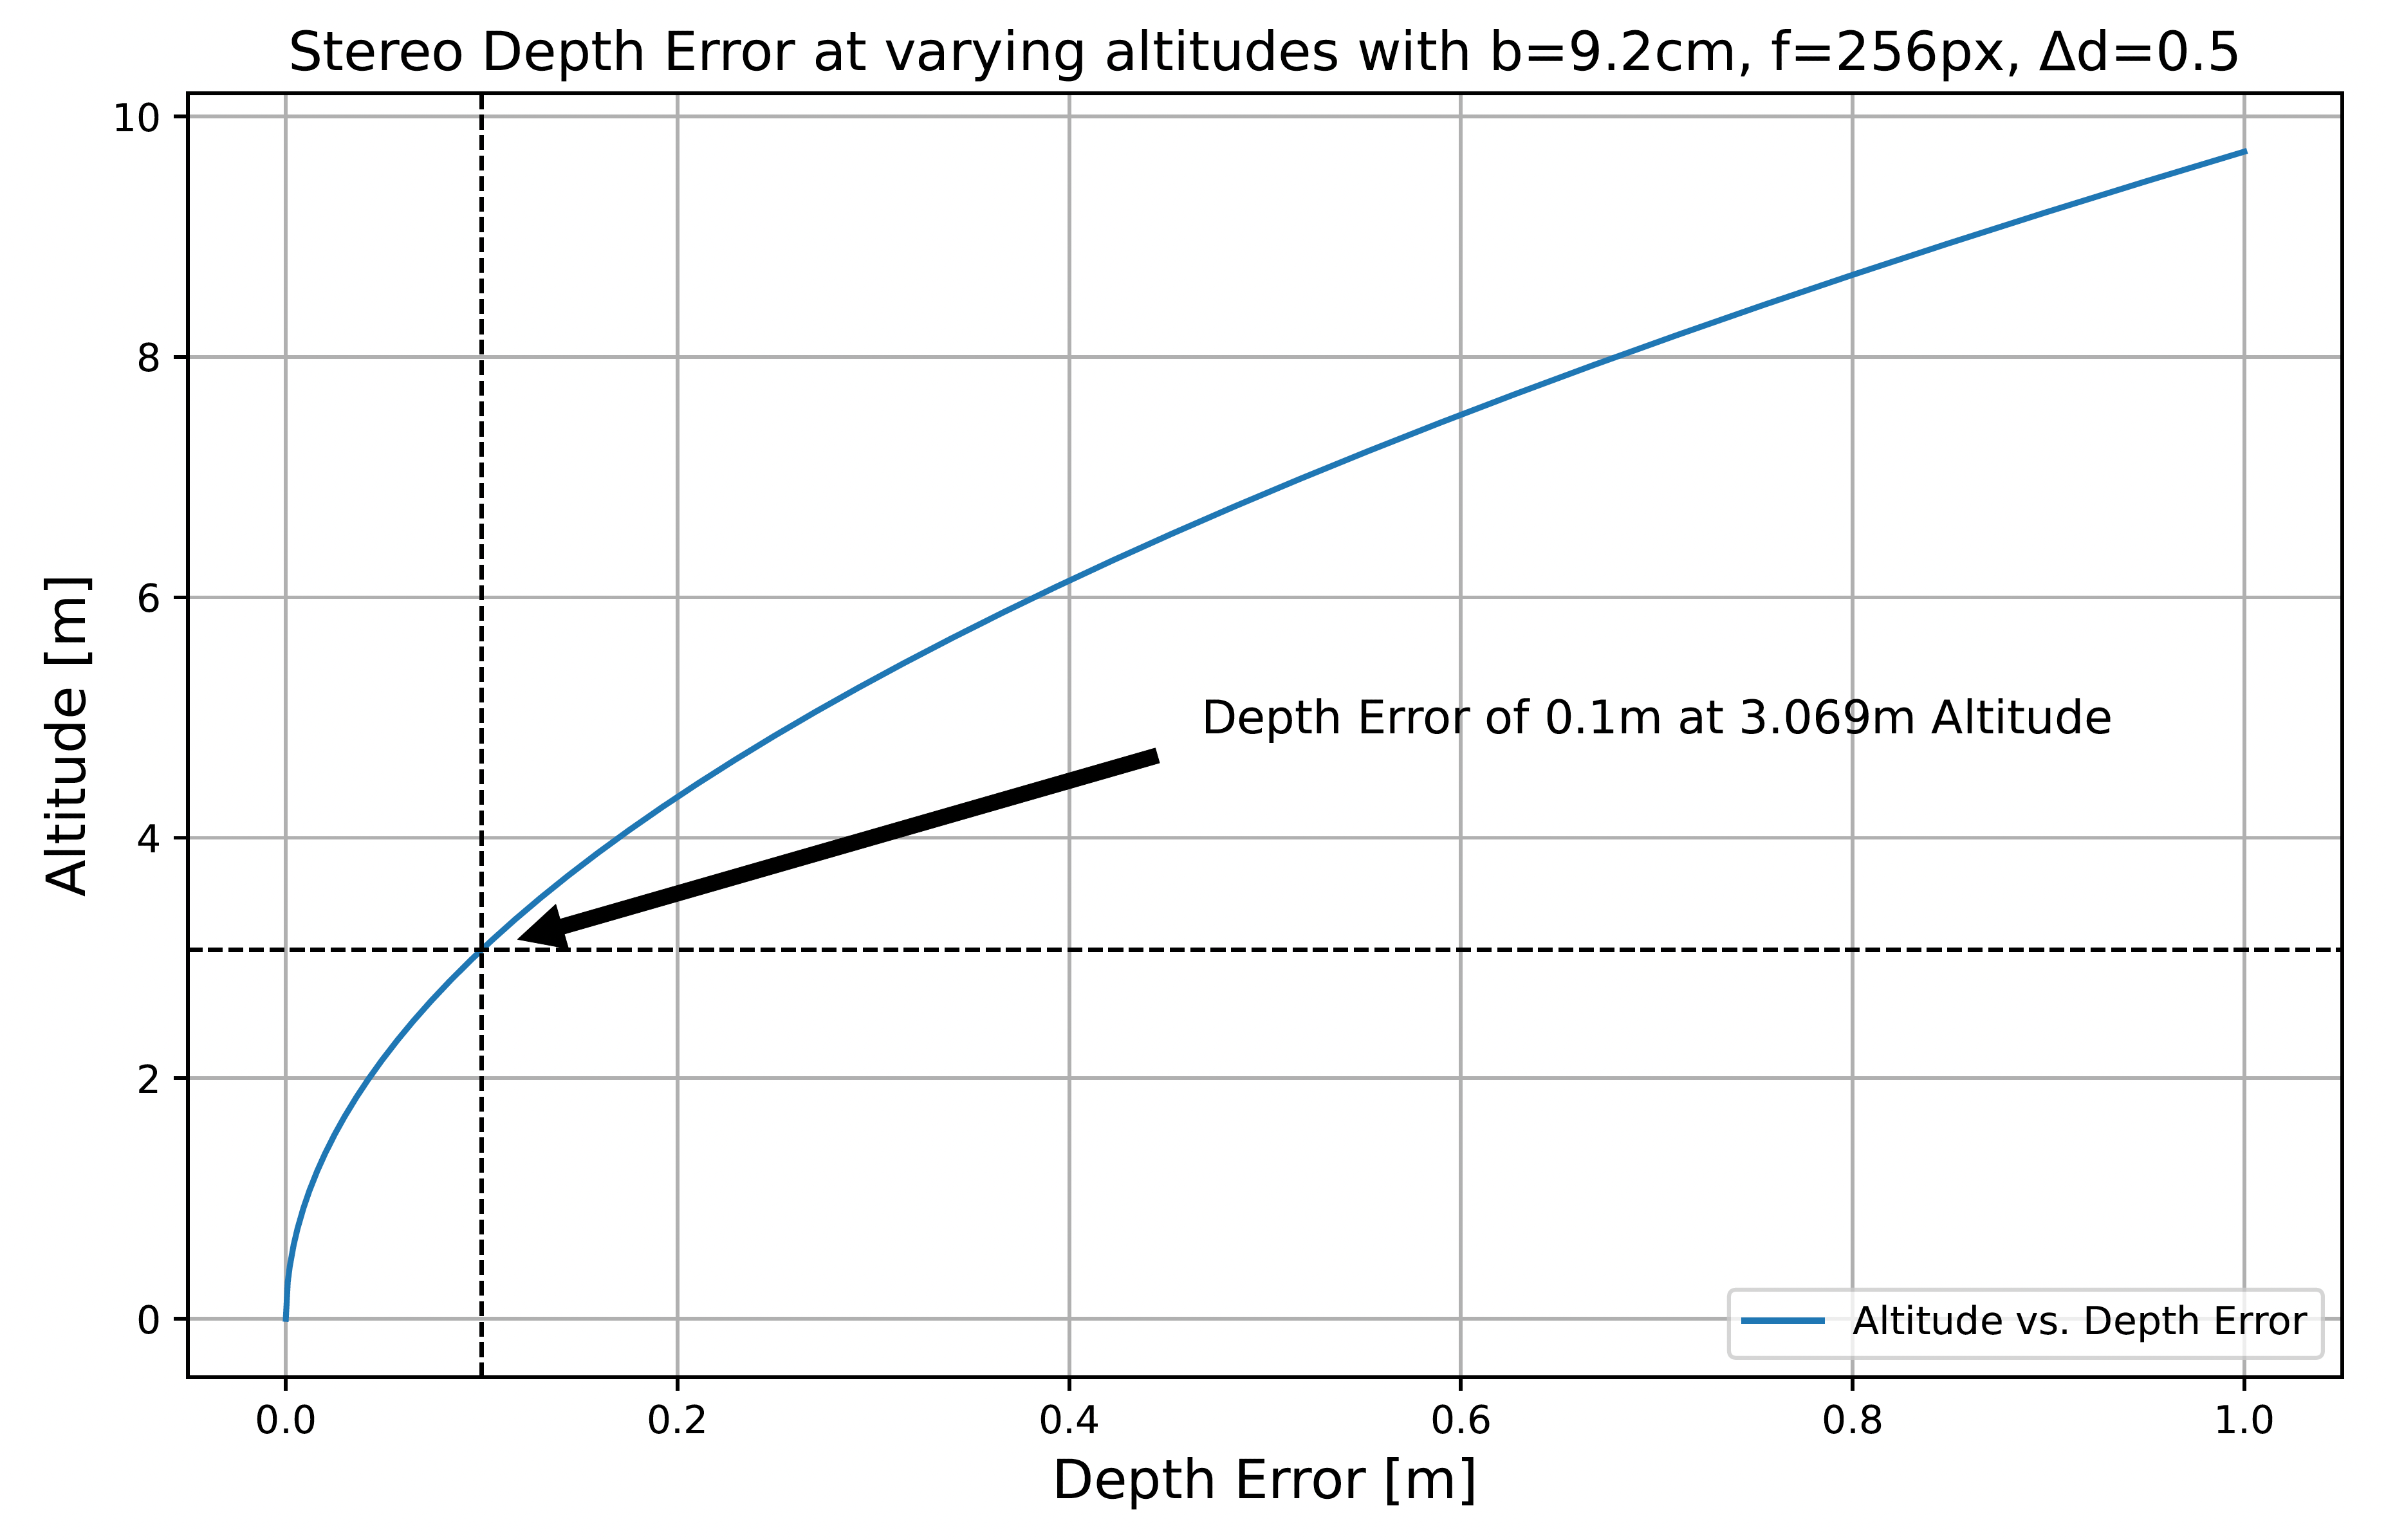
\includegraphics[scale=0.19]{images/preparation/stereo_limit.png}
    \label{fig:stereo_limit}
\end{figure}

Let's assume we allow a maximum depth error of 10cm. Considering this constraint we can fly at a maximum altitude of about 3m as indicated in \cref{fig:stereo_limit}.

This limitatin has to be kept in mind. However, it is neither too surprising nor is it too restrictive as the stereo camera is simply a depth alternative for low altitude flight maneuvers. In the context of an entire science mission it is almost exclusively used for landing site verification purposes.

\subsection{Implementation}

Like Structure from Motion, the stereo depth instance is a ROSnode which is given images and image poses from the xVIO state estimator. As the state estimator was in its final development stages during my thesis, camera images and a ground truth camera pose from the simulation were used instead as input for the stereo algorithm. Note that only one camera pose is given as the second one is derived in a straight forward manner, given the fixed baseline.

The stereo depth implementation was done using opencv's StereoSGBM algorithm. As stereo depth generation is a widely known topic I won't go into the details here.

The final output of the node is a generated pointcloud in the world frame together with two poses representing the camera locations of the generated pointcloud.

Taking off vertically with the drone in the simulation, the first landing site without lateral motion was found.

\begin{figure}
    \centering
    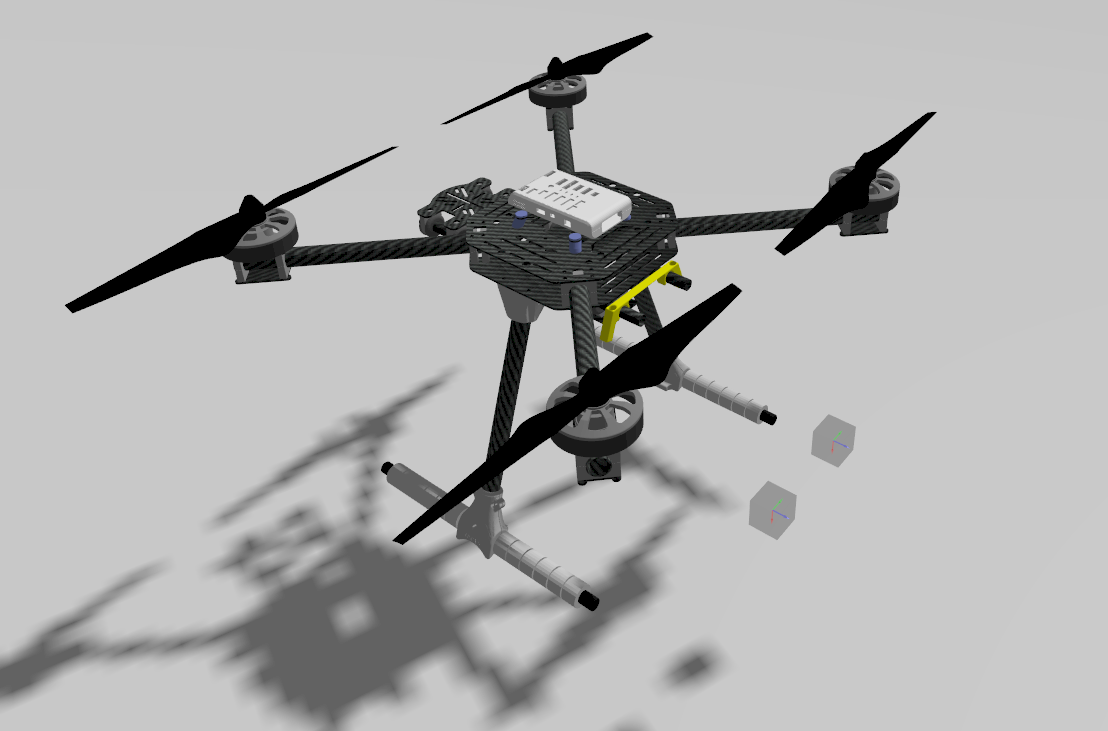
\includegraphics[scale=0.32]{images/preparation/stereo/drone_with_stereo_cam.png}
    \caption{Stereo camera on drone indicated by opaque boxes}
\end{figure}

\begin{figure}
    \centering
    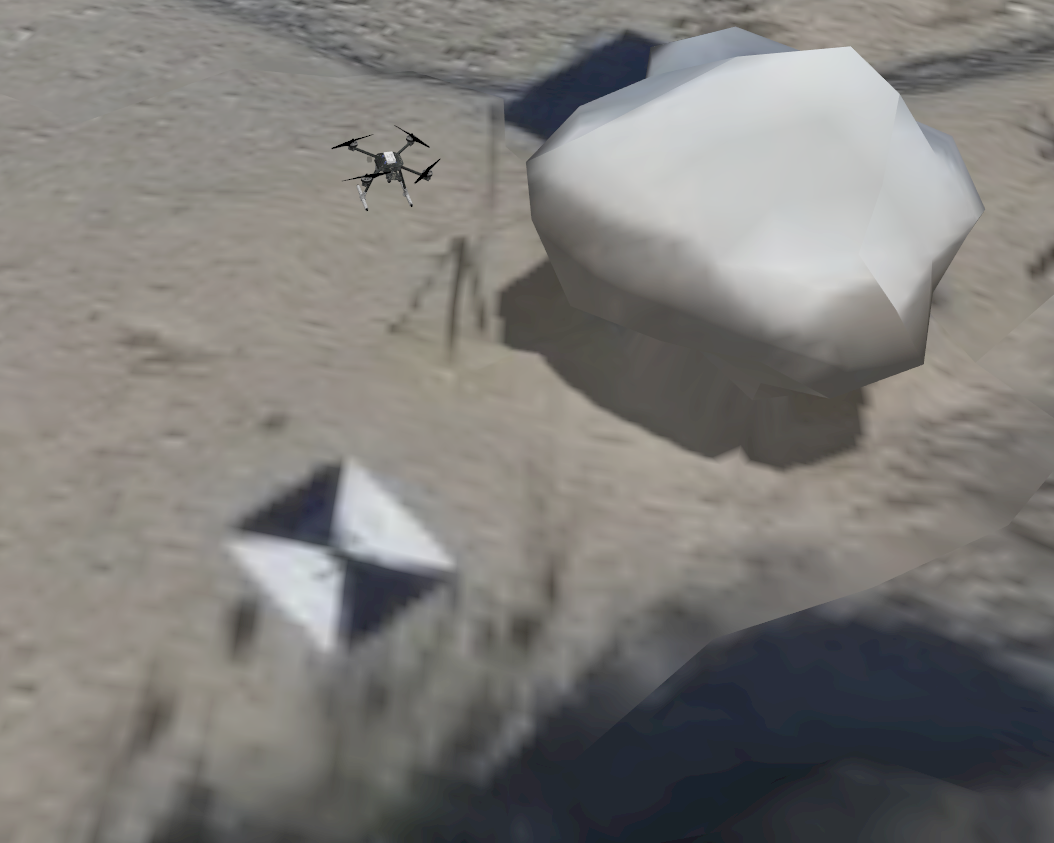
\includegraphics[scale=0.34]{images/preparation/stereo/ascent_sim.png}
    \caption{Drone during vertical ascent in simualation}
\end{figure}

\begin{figure}
    \centering
    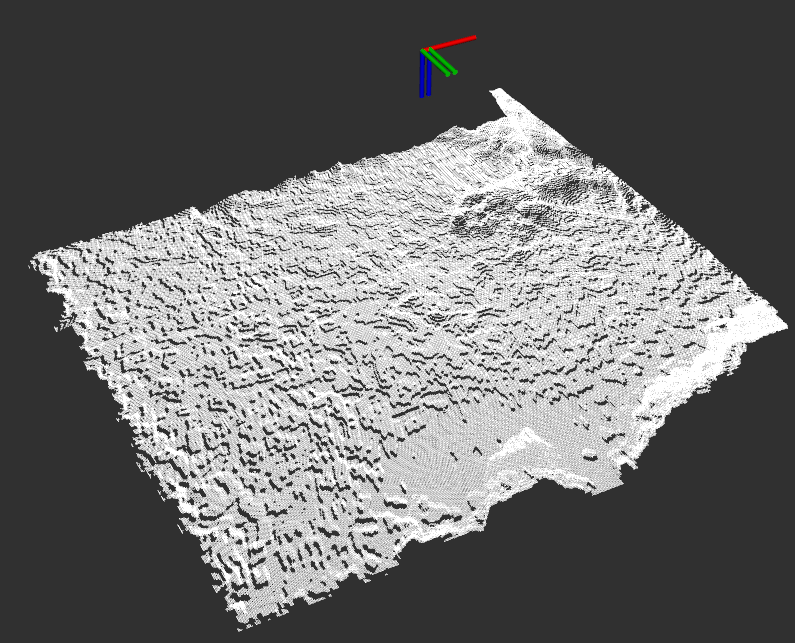
\includegraphics[scale=0.45]{images/preparation/stereo/stereo_pointcloud.png}
    \caption{Rviz visualization of created point cloud from stereo camera}
\end{figure}
\clearpage %HERE

\begin{figure}
    \centering
    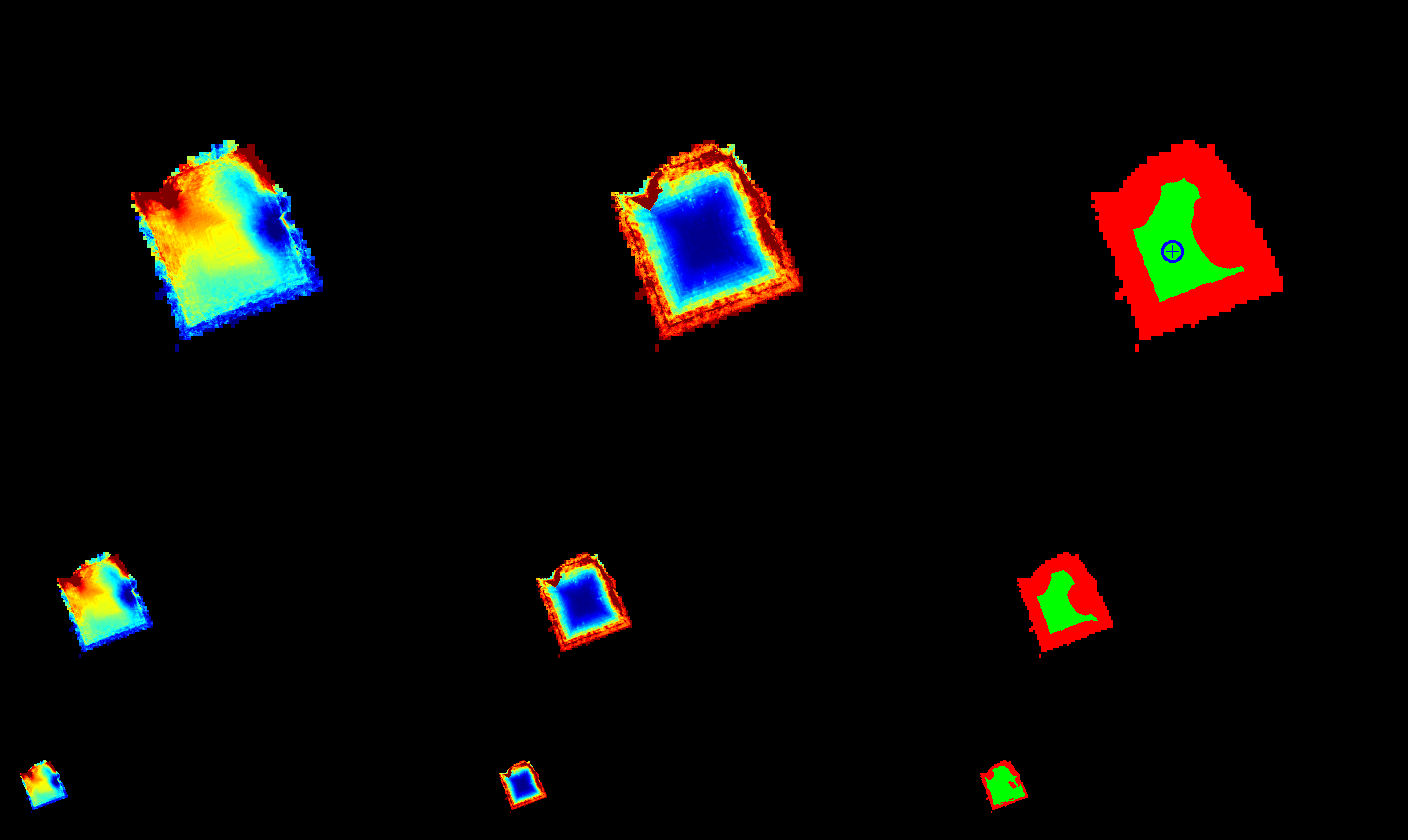
\includegraphics[scale=0.25]{images/preparation/stereo/lsd_ascent.png}
    \caption{LSD Debug output displaying LORNA's first detected landing site during vertical motion}
\end{figure}

\subsubsection{Switching}

In order to achieve the final desired perception mechanism of flying laterally with SFM and using a stereo camera depth node at low altitudes, one needs to switch between the two alternatives.

The obvious flag to use in the switching mechanism is the current altitude above ground. This could be achieved by analyzing the generated point cloud at a given iteration to the determine the median altitude which indicates the altitude above ground. This however is avoidable computational overhead.

As mentioned in \cref{sec:state_estimator} the drone has a laser range finder on board. This allows us to get an estimate of the altitude above ground at any given moment without the need for image processing.

Therefore, the switching is performed by using a separate ROSsubscriber which continuously checks the lrf's measurement and activates or deactivates the SFM node and stereo node respectively.

\clearpage %HERE
\begin{figure}
    \centering
    \includegraphics[scale=0.17]{images/preparation/stereo/switching.png}
    \caption{Laser Ranger Finder Based Switch between Depth Sources}
\end{figure}

\subsubsection{Qualitative Practical Analysis}

Once implemented the landing site detection instance could be supplied by the stereo depth node. The result thereof can be seen below:

\begin{figure}[ht!]
    \centering
    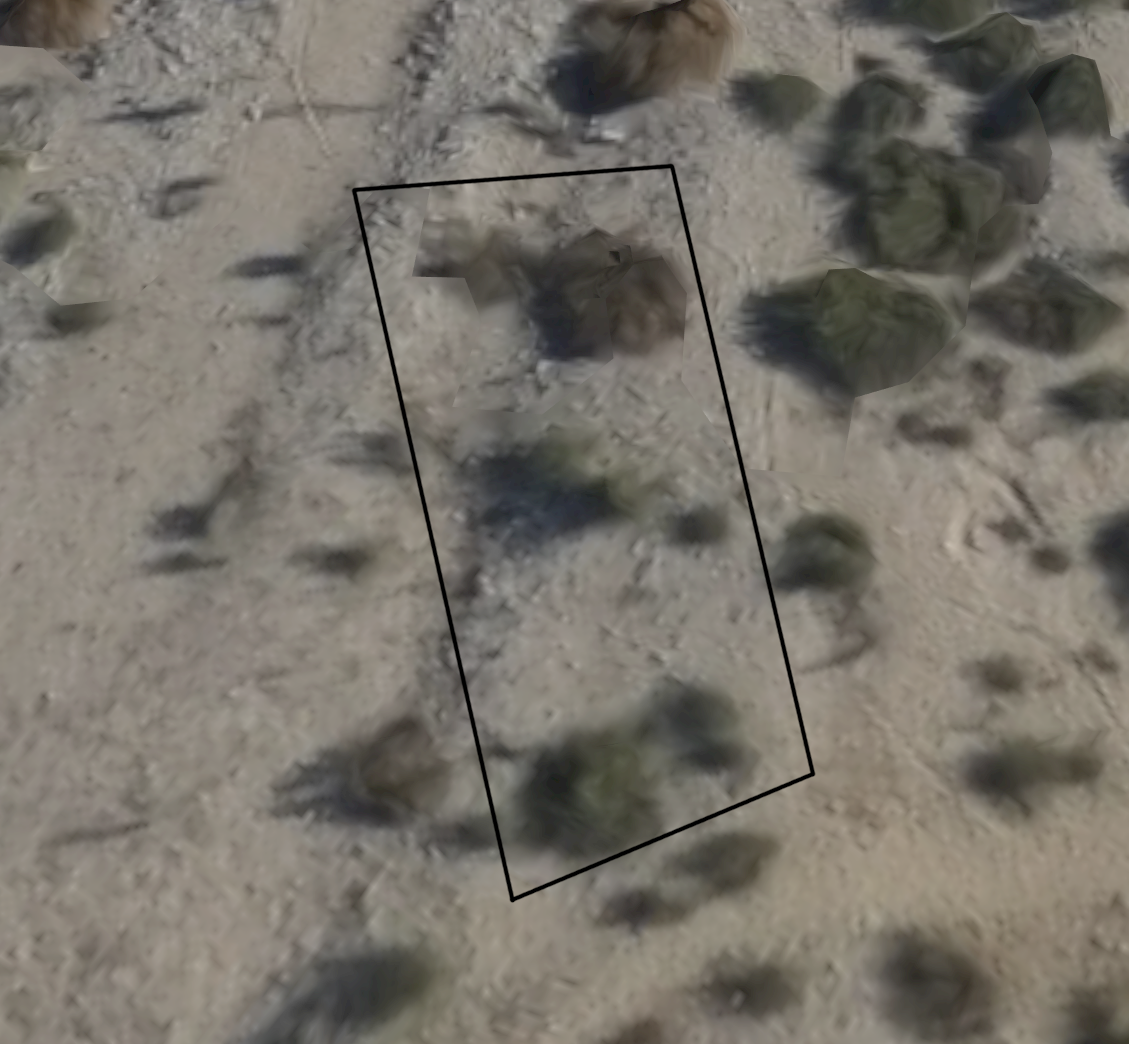
\includegraphics[scale=0.2, angle=-12]{images/preparation/reference_map2.5m_annotated.png}
    \caption{Considered terrain patch in Gazebo simulation}
    \label{stereo_reference}
\end{figure}

\begin{figure}[ht!]
    \centering
    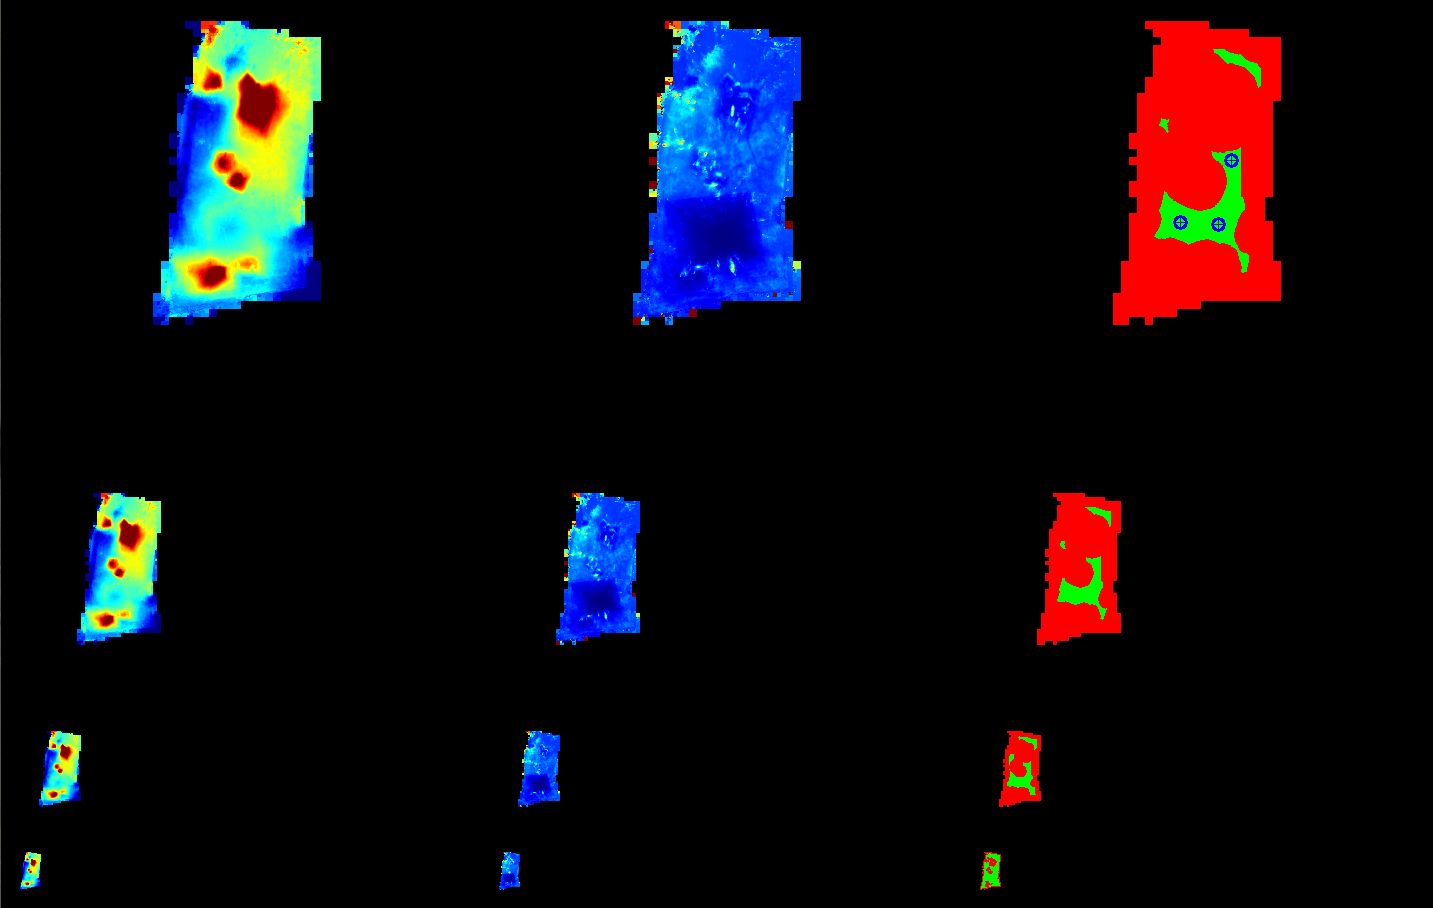
\includegraphics[scale=0.25]{images/preparation/stereo_2.5m.png}
    \caption{Stere camera depth supplied LSD debug image at 2.5m altitude}
    \label{qual_stereo_test}
\end{figure}

\clearpage %HERE

\begin{figure}[ht!]
    \centering
    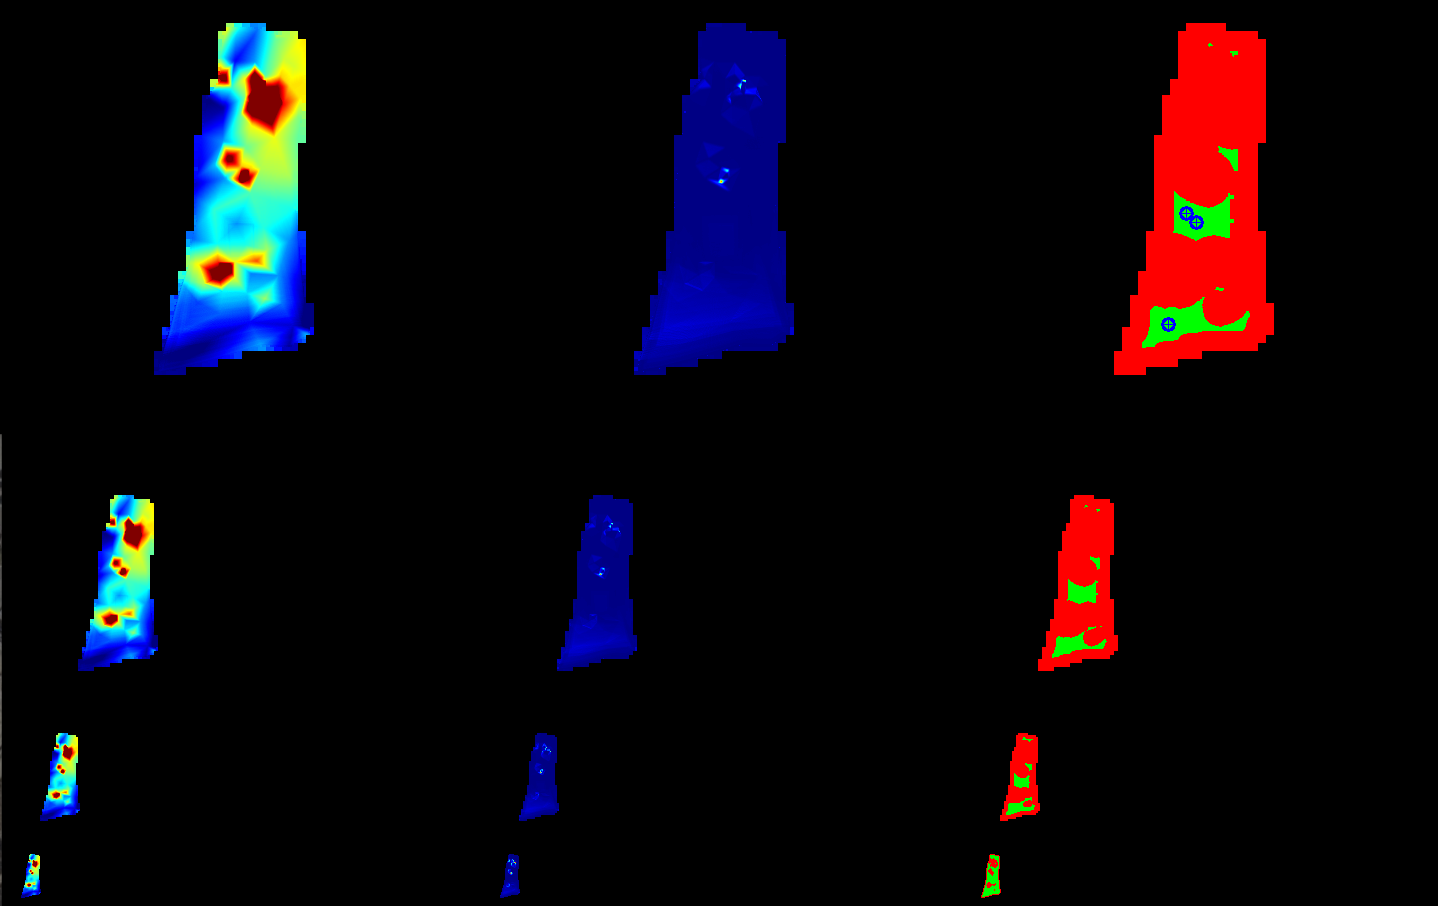
\includegraphics[scale=0.25]{images/preparation/GT_2.5m.png}
    \caption{GT depth supplied LSD debug image at 2.5m altitude}
    \label{stereo_GT}
\end{figure}

When comparing the result to the ground truth LSD output it can be seen that LSD creates a very accurate DEM from the stereo camera depth input. The landing sites detected are reasonable when looking at the terrain reference. 

\section{Ground Truth Depth}

For evaluation purposes as well as proof of concept aspirations a ground truth is required. The simulation already supplied the ground truth pose of the drone's base link through the ROSbridges. When applying the static camera transform to it, this yielded the ground truth camera pose.

\subsection{Gazebo Garden Depth Camera}\label{subsec:gz_depth_camera}

Obviously the same approach could be taken for a point cloud created by a depth camera in the simulation. However, implementing such a depth camera with equal camera parameters as the reference stereo camera showed different results.


\begin{figure}[ht]
    \centering
    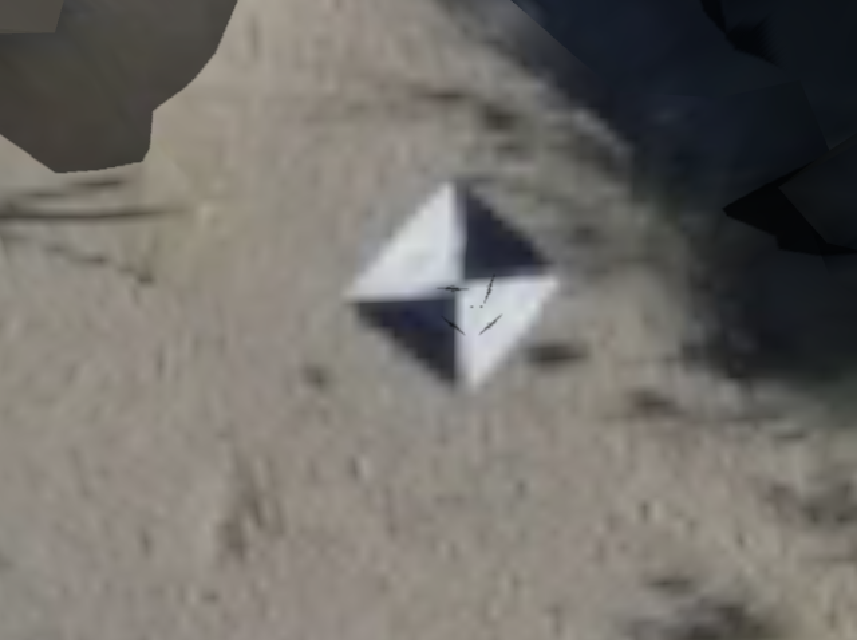
\includegraphics[scale=0.4]{images/preparation/GT_error_sim.png}
    \caption{Simulation Reference}
    \label{fig:GT_error_sim}
\end{figure}
\begin{figure}
    \centering
    
\includegraphics[scale=0.4]{images/preparation/GT_error_GT.png}
    \caption{GT depth image with wrong calibration}
    \label{fig:GT_error_GT}
\end{figure}

\clearpage %HERE

Looking at \cref{fig:GT_error_sim} and \cref{fig:GT_error_GT} the error looks like a simple translation error or is even hard to see at all. Focus for instance on the edge of the canape in the top left. When comparing the extrinsic parameters of the cameras, they were perfectly aligned. Further tests showed however that there was an actual error in the Gazebo Garden source code.\footnote[1]{For more footage on this see \cref{chapter:appendix:gz_depth_camera}} No matter what camera parameters were passed, the depth camera had the same fov. Changing this depth camera implementation finally allowed the usage of a gazebo depth camera as a supplier of ground truth depth information.

\section{Landing Site Properties}\label{sec:LSproperties}

With the low altitude depth alternative in place, the connection of the autonomy with the landing site detector could be tackled. 

Before this work the output of the landing site dection algorithm was merely the location of a found landing site. However, as described in \cref{subsubsec:setup:haz_seg} the landing site detection algorithms segments hazards based on roughness and slope. Subsequently it considers the size of a landing site as well as the uncertainty associated with a certain selected location. 

Simply outputting the location of a landing site is therefore a waste of information when so many characteristics are at hand to make an informed selection. 

I decided on the following properties to be output alongside the site's location:

\begin{itemize}
    \item Uncertainty
    \item Roughness
    \item Size
    \item Obstacle Altitude
\end{itemize}
The final landing site detection output is a custom landing site ROS message containing the above mentioned characteristics of the detected spot.

\subsection{Roughness}

The roughness value the exact value already used for the hazard segmentation step in the landing site detection. 

\subsection{Uncertainty}

The uncertainty value is also a product of the landing site detection algorithm. It denotes the averaged uncertainty across the area around a given landing site. The uncertainty of a single map cell denotes the stereo depth error estimates merged over time.

\subsection{Size}

To determine the size of a landing site, the landing site detection algorithm performs a distance transform on the created landing site map in order to find the closest non-landing site for any found landing site. This returns the radius of the largest valid landing circle around a landing site. Calculating the physical value, the metric radius is returned as the size of a landing site.

\subsection{Obstalce Altitude}\label{subsec:obstacle_altitude}

The obstacle altitude was newly introduced in this work. It defines the currently highest point of the aggregated DEM's highest resolution layer. As no actual object detection is performed and no hazard information is retained in this visual pipeline, this value serves the autonomy as an indication of the obstacles heights to avoid in the vicinity of a certain landing site. More on this in \cref{subsubsec:LandingSiteHeuristic}.



